\documentclass[handout]{beamer}
%Пакеты для математических символов:
\usepackage{amsmath} % американское математическое сообщество.
\usepackage{amssymb} % миллион разных значков и готический, ажурный шрифты.
\usepackage{amscd} % диаграммы, графики.
\usepackage{amsthm} % окружения теорем, определений и тд.
\usepackage{physics} % основные физические символы
%\usepackage{latexsym} % треугольники и пьяная стрелка.

%пакеты для шрифтов:
%\usepackage{euscript} % прописной шрифт с завитушками.
\usepackage{MnSymbol} % Значеки доказательства
\usepackage{verbatim} % улучшенный шрифт "пишущей машинки".
%\usepackage{array} % более удобные таблицы.
%\usepackage{multirow} % мультистолбцы в таблицах.
%\usepackage{longtable} % таблицы на несколько страниц.
%\usepackage{latexsym}

\usepackage{etoolbox}
\usepackage{slashbox} %Разделениени текста \backslashbox{}{}
\usepackage{collectbox} % Добавляет коробочки, можно складывать туда текст)

%Пакеты для оформления:
\RequirePackage[center, medium]{titlesec}% Стиль секций и заголовков
%\usepackage[x11names]{xcolor} % 317 новых цветов для текста.
%\usepackage{multicol} % набор текста в несколько колонн.
%\usepackage{breqn} % мультистоки в урвнениях 
\usepackage{graphicx} % расширенные возможности вставки стандартных картинок.
\usepackage{subcaption} % возможность вставлять картинки в строчку
%\usepackage{caption} % возможность подавить нумерацию у caption.
\usepackage{wrapfig} % вставка картинок и таблиц, обтекаемых текстом.
\usepackage{cancel} % значки для сокращения дробей, упрощения, стремления.
%\usepackage{misccorr} % в заголовках появляется точка, но при ссылке на них ее нет.
%\usepackage{indentfirst} % отступ у первой строки раздела
%\usepackage{showkeys} % показывает label формул над их номером.
%\usepackage{fancyhdr} % удобное создание верхних и нижних колонтитулов.
%\usepackage{titlesec} % еще одно создание верхних и нижних колонтитулов

%Пакеты шрифтов, кодировок. НЕ МЕНЯТЬ РАСПОЛОЖЕНИЕ.
\usepackage[utf8]{inputenc} % кодировка символов.
%\usepackage{mathtext} % позволяет использовать русские буквы в формулах. НЕСОВМЕСТИМО С tempora.
\usepackage[T1, T2A]{fontenc} % кодировка шрифта.
\usepackage[english, russian]{babel} % доступные языки.


%Отступы и поля:
%размеры страницы А4 11.7x8.3in
\textwidth=7.3in % ширина текста
\textheight=10in % высота текста
\oddsidemargin=-0.5in % левый отступ(базовый 1дюйм + значение)
\topmargin=-0.5in % отступ сверху до колонтитула(базовый 1дюйм + значение)


%Сокращения
\newcommand{\piv}[2]{\cfrac{\partial #1}{\partial #2}}


%Скобочки
\newcommand{\inrad}[1]{\left( #1 \right)}
\newcommand{\inner}[1]{\left( #1 \right)}
\newcommand{\infig}[1]{\left{ #1 \right}}
\newcommand{\insqr}[1]{\left[ #1 \right]}
\newcommand{\ave}[1]{\left\langle #1 \right\rangle}


%% Красивые <= и >=
\renewcommand{\geq}{\geqslant}
\renewcommand{\leq}{\leqslant}

%%Значек выполнятся
\newcommand{\per}{\hookrightarrow}


%% Более привычные греческие буквы
\renewcommand{\phi}{\varphi}
\renewcommand{\epsilon}{\varepsilon}
\newcommand{\eps}{\varepsilon}
\newcommand{\Eps}{\mathfrak{E}}
\newcommand{\com}{\mathbb{C}}
\newcommand{\re}{\mathbb{R}}
\newcommand{\nat}{\mathbb{N}}
\newcommand{\stp}{$\filledmedtriangleleft$}
\newcommand{\enp}{$\filledmedsquare$}

\makeatletter
\newcommand{\sqbox}{%
    \collectbox{%
        \@tempdima=\dimexpr\width-\totalheight\relax
        \ifdim\@tempdima<\z@
            \fbox{\hbox{\hspace{-.5\@tempdima}\BOXCONTENT\hspace{-.5\@tempdima}}}%
        \else
            \ht\collectedbox=\dimexpr\ht\collectedbox+.5\@tempdima\relax
            \dp\collectedbox=\dimexpr\dp\collectedbox+.5\@tempdima\relax
            \fbox{\BOXCONTENT}%
        \fi
    }%
}
\makeatother
\newcommand{\mergelines}[2]{
\begin{tabular}{llp{.5\textwidth}}
#1 \\ #2
\end{tabular}
}
\newcommand\tab[1][0.51cm]{\hspace*{#1}}
\newcommand\difh[2]{\frac{\partial #1}{\partial #2}}


\usetheme{Madrid} % Выбор темы
\usecolortheme{seahorse} % Выбор цветовой схемы
\title{Генерация гармоник высокого порядка (ГГВП)}
\author{Карибджанов Матвей}

\begin{document}



\begin{frame}% первый слайд
    \titlepage
\end{frame}

\begin{frame}
    \frametitle{Обнаружение}
    \begin{figure}[h]
        \centering
        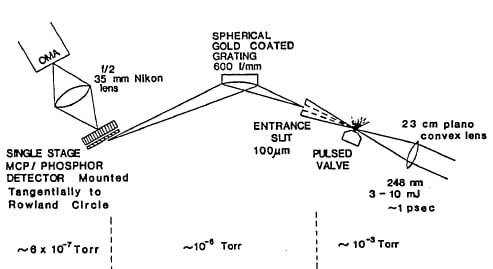
\includegraphics[width=1\textwidth]{Mc/ex_1.jpg}
    \end{figure}
\end{frame}


\begin{frame}
    \frametitle{Параметры системы}
    \begin{columns}
        \begin{column}{0.3\textwidth}
            Параметры системы:
            \begin{itemize}
                \item $\mathfrak{J} \sim 10^{15} W/cm^2$
                \item $n \sim 10^{18} cm^{-3}$
                \item $p \approx 3.1 \cdot 10^4 Torr$
                \item $T > 350 fs$
                \item $\lambda 248 nm$
            \end{itemize}
        \end{column}

        \begin{column}{0.7\textwidth}
            \begin{figure}[h]
                \centering
                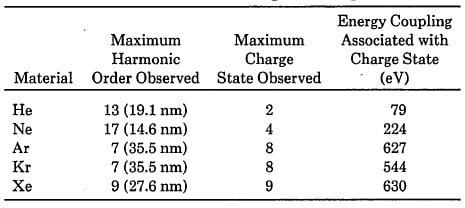
\includegraphics[width=1\textwidth]{Mc/samp_max_n.jpg}
            \end{figure}
        \end{column}
      \end{columns}
\end{frame}

\begin{frame}
    \frametitle{Результаты}
    \begin{columns}
        \begin{column}{0.5\textwidth}
            \begin{figure}[h]
                \centering
                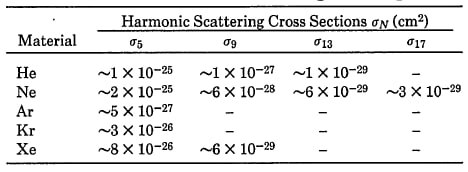
\includegraphics[width=1\textwidth]{Mc/samp_n.jpg}
            \end{figure}
            \begin{equation}
                \eps = \eps_i + 3 U\inner{\mathfrak{J}}
            \end{equation}
        \end{column}

        \begin{column}{0.5\textwidth}
            \begin{figure}[h]
                \centering
                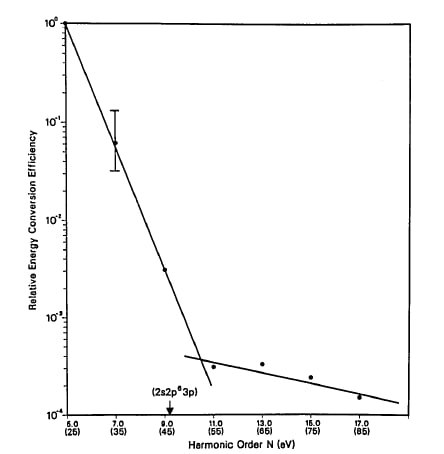
\includegraphics[width=1\textwidth]{Mc/n_I.jpg}
            \end{figure}
        \end{column}
      \end{columns}
\end{frame}

\begin{frame}
    \frametitle{Модель 1}
    \begin{columns}
        \begin{column}{0.5\textwidth}
            Подгоночная модель
            \begin{equation}
                \eps = \eps_i + U_e
            \end{equation}
            \begin{equation*}
                \ddot x = - \cfrac{e}{m}E \cos\inner{\omega t}
            \end{equation*}
            \begin{align*}
                x = \cfrac{eE}{m\omega \tau } [\inner{t_r - t} \cos t_r \omega + \\
                + \inner{t - t_i} \cos t_i \omega + \tau \cos t \omega]
            \end{align*}
            Где
            \begin{equation*}
                \tau = t_r - t_i
            \end{equation*}    
            \begin{equation}
                \eps = \cfrac{m \dot x (t_r)}{2} = 3.17 U
            \end{equation}
        \end{column}
        
        \begin{column}{0.5\textwidth}
            \begin{figure}[h]
                \centering
                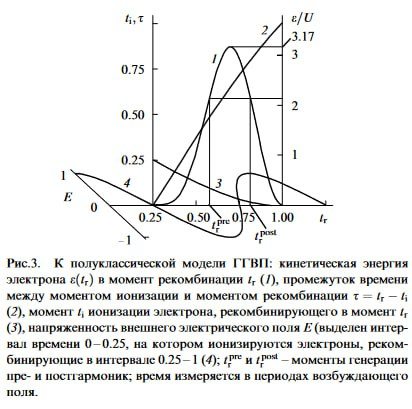
\includegraphics[width=1\textwidth]{new/approx.jpg}
            \end{figure}
        \end{column}
      \end{columns}
\end{frame}

\begin{frame}
    \frametitle{Модель 2}
    \begin{columns}
        \begin{column}{0.5\textwidth}
            Квантовомеханическая модель
            \begin{equation}
                i h \piv{\phi}{t} = \inner{\cfrac{p^2}{2m} + U + H^{int}}\phi 
            \end{equation}
            В простейшем случае
            \begin{equation}
                U = \alpha \delta r, \ H^{int} = erE
            \end{equation}
            Бывают модели 
            \begin{equation}
                U = \cfrac{e^2Z}{r}, \ H^{int} = pmA + \cfrac{e^2 A^2}{2mc^2}
            \end{equation}
            
        \end{column}
        
        \begin{column}{0.5\textwidth}
            \begin{equation*}
                \phi = \phi_0 + \phi_1
            \end{equation*}
            $\phi_0$ - связанный, $\phi_1$ - свободный электрон.

            \begin{align*}
                \ket{\phi_0 + \phi_1} = \\
                \frac{1}{ih} \int_{\infty}^{t} d\tau \int d^3 p
                \exp\inner{-\frac{i}{h} \int_\tau^{t} E_p dt} \\
                \times \ket{\phi_p}\bra{\phi_p}V\ket{\phi_0(\tau)}
            \end{align*}
            \begin{equation*}
                \phi_p = \inner{2\pi h}^{3/2} \exp\inner{i/h pr}
            \end{equation*}
            Критерий приближения $WT \ll 1$
        \end{column}
      \end{columns}
\end{frame}

\begin{frame}
    \frametitle{Современные методы}

    \begin{columns}
        \begin{column}{0.4\textwidth}
            \begin{itemize}
                \item $n \sim 3\cdot 10^{16} - 3\cdot 10^{18} cm^{-3}$
                \item $\lambda = 1.05 - 0.388 \mu m$
                \item $T = 25 - 800 fs$
                \item $\mathfrak{J} \sim 10^{14} - 10^{18}  W/cm^2$
            \end{itemize}
        \end{column}
        
        \begin{column}{0.7\textwidth}
            \begin{figure}[h]
                \centering
                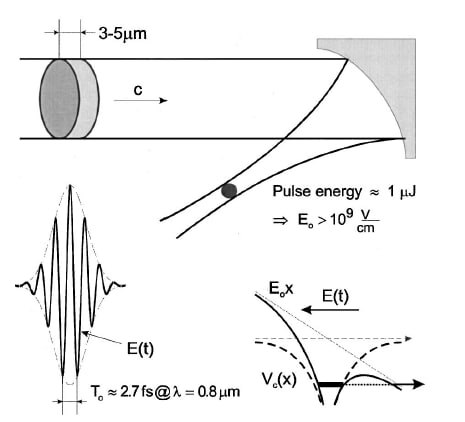
\includegraphics[width=0.8\textwidth]{new/new_ex.jpg}
            \end{figure}
        \end{column}
      \end{columns}
\end{frame}

\begin{frame}
    \frametitle{Результаты предсказания модели}

    \begin{columns}
        \begin{column}{0.5\textwidth}
            \begin{figure}[h]
                \centering
                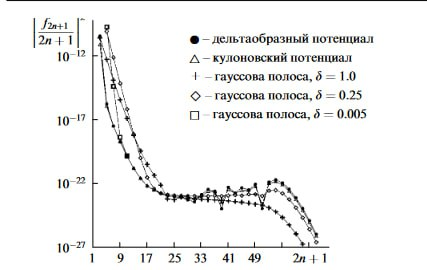
\includegraphics[width=1\textwidth]{new/theor_samp.jpg}
            \end{figure}
        \end{column}
        
        \begin{column}{0.5\textwidth}
            \begin{figure}[h]
                \centering
                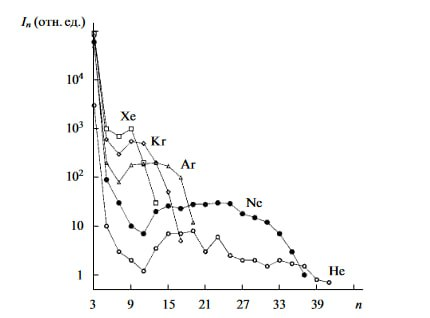
\includegraphics[width=1\textwidth]{new/samp.jpg}
            \end{figure}
        \end{column}
      \end{columns}
\end{frame}

\begin{frame}
    \frametitle{Список литературы}
    \begin{itemize}
        \item В. Т. Платоненко, В. В. Стрелков, Генерация гармоник высокого порядка в
        поле интенсивного лазерного излучения, Квантовая электроника, 1998, том 25,
        номер 7, 582–600 (Теория)
        \item Б. В. Румянцев, А. В. Пушкин, Ф. В. Потёмкин, Генерация гармоник высокого порядка вблизи низкочастотного края
        плато при нелинейном распространении фемтосекундного лазерного
        излучения ближнего ИК диапазона с длиной волны 1.24 мкм
        в плотной струе аргона
        \item Thomas Brabec and Ferenc Krausz, Intense few-cycle laser fields: Frontiers of nonlinear optics, 545-585
        \item McPherson A., Gibson G., Jara H., Johann U., Luk T.S., McIntyre
        I.A., Boyer K., Rhodes C.K. J.Opt.Soc.Amer. B, 4, 595 (1987). (Первый эксперимнет с хорошим описнием)
    \end{itemize}
\end{frame}

\end{document}